

\chapter{Marco Te\'orico}
\label{cap:preliminares}

\section{Impresión 3D}

 A diferencia de las técnicas principales que se emplean desde hace algunos años en la fabricación de objetos, que se encargan de sustraer, combinar, o deformar paulatina y controladamente materia hasta llegar a una pieza final, la impresión 3D funciona de un modo completamente distinto. La pieza se crea en un solo paso, capa por capa, a un ritmo medio de uno a dos centímetro de altura por hora; el objeto creado puede constar de mecanismos internos (como rodamientos de bolas), formas tejidas y entrelazadas, o incluso huecos y curvas \citep{Berchon2014}. Pues bien, todas las impresoras 3D, están basadas sobre el mismo principio: un modelo digital es transformado a un objeto físico de 3 dimensiones por adición de material en capas. Esto se conoce alternativamente como \textit{Manufactura Aditiva} \citep{tresdhub2018}. Este tipo de fabricación también se puede englobar dentro de lo que se denomina \textit{Fabricación digital}, cuyo principio básico es la transformación de la información  desde el mundo físico al digital. Según \citep{jorquera2016}, la fabricación digital incluye los siguientes sistemas y tecnologías:\\
 
 \begin{enumerate}
 	
	\item Sistemas integrados: Es un \textit{hardware} electrónico diseñado específicamente para llevar a cabo una o pocas tareas definidas. Las impresoras llevan un sistema electrónico integrado que utilizan para controlar los motores paso a paso que alimentan el papel, recibir información de los sensores de temperatura y finales de carrera, o que mandan al cabezal de impresión.
	\item Sistemas CNC (\textit{Computer Numeric Control} - control numérico computarizado): Es el control numérico de un sistema de automatización que se utiliza para controlar diferentes máquinas herramienta. Este sistema ha revolucionado la industria gracias a la simplificación del \textit{software} de diseño en conjunto con los lenguajes de programación como el \textit{.gcode}. Esencialmente, un sistema CNC es cualquier sistema que utiliza un ordenador para controlar los movimientos de una máquina.
	\item Software CAD (\textit{Computer Aided Design}- diseño asistido por computador): es, en esencia, un programa que sirve para la creación, edición análisis y visualización de modelos tridimensionales.  
	\item Internet: Los programas CAD actuales disponen de herramientas de trabajo colaborativo en red, de esta manera se define el producto y el proceso de fabricación de forma simultánea.\\

  \end{enumerate}

En la misma línea, y dependiendo de la profundidad técnica que el proceso de fabricación necesite, se agregan los sistemas \citep{leao2017}:

\begin{enumerate}
	\item Software CAE (\textit{Computer Aided Engineering} - Ingeniería Asistida por computador): Son los programas mayoritariamente usados para las tareas de análisis de ingeniería. Estos \textit{softwares}, a través de métodos numéricos como el método de elementos finitos o dinámica de fluidos computacional, se utilizan para, por ejemplo, analizar la robustez y el funcionamiento de ensambles de piezas.
	\item Software CAM (\textit{Computer Aided Manufacturing}- Manufactura Asistida por computador): Corresponde a programas que controlan las herramientas de máquinas de control numérico relacionadas con el proceso de manufactura a realizar, generando un código específico para el producto a fabricar. 

\end{enumerate}



\subsection{Historia de la impresión 3D}

La primera vez que se hizo pública la conceptualización de algo que pudiese parecerse a una impresora 3D, se remonta al año 1964, cuando el científico y escritor británico Arthur C. Clarke realiza la descripción de una máquina ficticia llamada \textit{El Replicador}. En teoría, este artefacto -que en palabras del autor \textit{es la invención que va a poner fin todas las invenciones}- sería capaz de crear una copia exacta de una cosa, reorganizando partículas subatómicas, y luego ensamblar esas moléculas para ser transformadas en un objeto real \citep{renstrom2012}. No obstante, el comienzo de la generación del concepto técnico de impresión 3D puede ser rastreado al año 1976, a partir de la creación de la primera impresora a tinta por inyección \citep{maxey2013}. La utilización de la inyección de tinta abrió la pregunta respecto a qué tipo de materias primas podían ser utilizadas con esta tecnología, y cómo los mecanismos presentes en la época podían ser adaptados para abrir la posibilidad de ocupar otras materias primas. En Mayo de 1981, el Dr. Hideo Kodama del Instituto de Investigación Industrial del Municipio de Nagoya publicó detalles relativos a la técnica de prototipado rápido. Esta investigación se considera como la primera publicación que describe la técnica de fabricación capa a capa propia de los procesos de impresión 3D; no obstante, los desarrollos de Kodama no llegaron a ser materializados debido a problemas encontrados en el proceso de fundido de material. \citep{tresdsourced2020}. Paralelamente, la idea de \textit{máquinas de prototipado rápido} continuó su desarrollo en Francia, por Jean-Claude André, Oliver de Witte y Alain le Méhauté. En la primera mitad de la década de los 80, le Méhauté investigaba en la empresa Alcatel sobre partes y piezas generadas a partir de la geometría fractal, y la manera en que éstas podrían ser fabricadas dada su complejidad de forma.
De Witte, quien era también investigador de Alcatel en el área de luz láser, propuso a le Méhauté que algunos líquidos compuestos por ciertos monómeros podían ser curados y transformados en sólidos tras la aplicación de luz láser, convirtiéndose en el primer paso para la construcción efectiva de máquinas de prototipado rápido a través de el proceso de Estereolitografía. Ambos compartieron el resultado de sus avances con André, que en ese tiempo trabajaba en el Centro Nacional Francés de Investigación Científica, para ya el año 1984 inscribir la patente de su desarrollo. Infortunadamente, el grupo debe abandonar el proyecto debido a problemas con la solidificación del material y poca rentabilidad desde la perspectiva económica \citep{alltresdp2018}.\

Con solo tres semanas de diferencia respecto a los investigadores franceses, Charles Hull, ingeniero graduado de la Universidad de Colorado, solicita la patente del proceso de Esterolitografía con nuevos avances, como la utilización del formato STL (Standard Triangle Language) y la laminación digital de objetos. A diferencia del a Esterolitografía francesa, el método de Hull utiliza luz ultravioleta para el curado de fotopolímeros. El año 1986, obtenida su patente, Hull forma la empresa \textit{3D Systems} y lanza la primera impresora 3D, la \textit{SLA-1}, el año 1987 \citep{tresdsourced2020}. Casi al mismo tiempo, la tecnología de modelado por deposición fundida (FDM) era patentada por Scott Crump como otra tecnología de fabricación aditiva\citep{alltresdp2018}. FDM utiliza un cabezal móvil, el cual funde un filamento de material qie se deposita en una plataforma. Es interesante mencionar que tanto las máquinas SLA como FDM son actualmente las más utilizadas y diversificadas en el mundo de la impresión 3D.
Un año después de la presentación de la SLA-1, Carl Deckard de la Universidad de Texas patentó la tecnología de Sinterizado Selectivo por Láser (SLS). En lugar de utilizar luz ultravioleta, SLS hace uso de un láser para trazar y solidificar las capas de un polvo de polímeros \citep{tresdsourced2020}. Así, la máquina de Deckard se convirtió en la primera impresora 3D en utilizar la tecnología SLS, a la cual llamó Betsy; sin embargo, el propósito central de su invención era testear el sistema de sinterizado por láser, por lo que la calidad de impresión y el nivel de detalle no estaba dentro de sus prioridades\citep{alltresdp2018}. 
En 1993, el MIT desarrolla una técnica de impresión 3D basada en las impresoras de inyección de tinta. Adaptando ésta a un movimiento en un nuevo eje, se crea la Z Corp Z402. El primero modelo utilizaba polvos basados en yeso como base y un aglutinante basado en agua. El mismo año, Royden Sanders fundó Solidscape, creando una impresora 3D basada en cera.
La segunda mitad de los años noventa vio la diversificación de las tecnologías para la técnica de fabricación aditiva, ampliando la gama de materias primas a utilizar y los proceso de transformación de materiales. En 1997, se crea la impresora 3D de metales, la cual utiliza el proceso de fundición por haz de electrones (EBM) y el perfeccionamiento del Polyjet. Así, este desarrollo trajo consigo mayores oportunidades comerciales para estas máquina abriéndose, entre otras, a la industria médica con la bioimpresión de partes adaptables al cuerpo humano tales como piezas dentales o prótesis\citep{tresdsourced2020}.
Los avances de las investigaciones y la búsqueda de la competitividad en la utilización de la impresión 3D como  manufactura aditiva trajo consigo durante los años posteriores el comienzo de la democratización de esta tecnología. Como se ha mostrado en esta sección, la impresión 3D es una tecnología que nace en los años ochenta, por lo cual es factible preguntar cómo y por qué estas máquinas son tan conocidas y valoradas en la actualidad, y de qué manera comienzan a gestar una de las mayores revoluciones tecnológicas del siglo XXI. El proyecto \textit{RepRap} nace el año 2005 a través de un blog impulsado por el doctor Adrian Bowyer, profesor de ingeniería mecánica de la Universidad de Bath del Reino Unido. En él, Bowyer comienza a modelar el primer boceto de una impresora 3D FDM con el objetivo de crear una máquina autoreplicante, capaz de imprimir nuevos componentes en 3D para ser útil en el desarrollo del prototipado rápido, y al mismo tiempo fabricar nuevas piezas para nuevas máquinas. Así, cualquier persona al otro lado del mundo y con las instrucciones adecuadas podría llegar a construirla  \citep{torre2013}. Según Torre (2013) a casi tres años del primer modelo, la \textit{RepRap 0.1} ya había impreso casi la mitad de sus propios componentes; al año 2008, se estima que ya existían más de 100 copias construidas y funcionando en todo el mundo. RepRap es un diseño abierto, y toda la propiedad intelectual producida en este proyecto está sujeto a una licencia de software libre \citep{alltresdp2016}. A partir de esta invención libre, y sumado al vencimiento de las patentes de las tecnologías SLA y FDM, se desata el desarrollo de nuevas impresoras como las de tipología Delta (no cartesiana), y la creación de empresas dedicadas a la fabricación de máquinas de bajo costo como MakerBot \citep{tresdsourced2020}. En la actualidad, se estima que el tamaño del mercado es de alrededor de 10 billones de dólares, y se espera que crezca alrededor de un 23,5\% anualmente, abarcando industrias como la automovilística, aeroespacial, médica, e inclusive el calzado deportivo\citep{donovan2019}.

\begin{figure}[H]
\centering
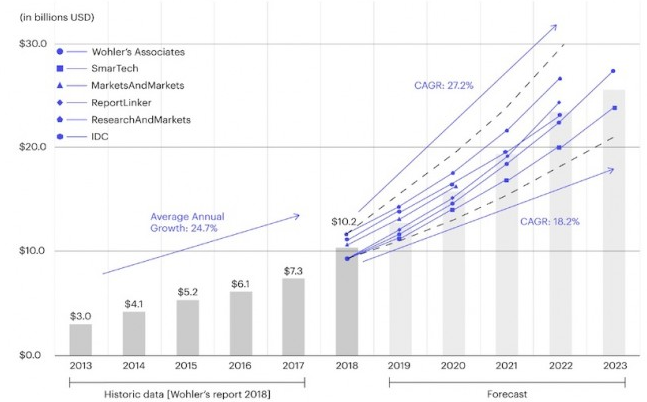
\includegraphics[scale=0.8]{images/3dmarket.png}
\caption{Tamaño del mercado y pronóstico de la impresión 3D \citep{donovan2019}.}

\end{figure}

\subsection{Métodos de impresión 3D}




\subsection{Impresoras 3D FDM}

\subsection{Tipologías de impresión 3D FDM}

\section{Mantenimiento}

Habitualmente, el concepto de mantenimiento puede definirse según distintas formas según el enfoque que se dé en cada caso. Un punto de partida, es mantener el correcto estado funcional de los equipos e instalaciones, sin embargo, las consecuencias que el desarrollo de este principio elemental puede tener sobrepasan ampliamente el objetivo inicial \citep{gomez1998}. En este sentido, y buscando una definición global, se puede decir que el mantenimiento corresponde al conjunto de técnicas destinado a conservar equipos e instalaciones en servicio durante el mayor tiempo posible (buscando la más alta disponibilidad) y con el máximo rendimiento \citep{garcia2010}.
Teniendo en cuenta factores como el tipo de industria y su tamaño, la política de la empresa, las características de la producción, el campo de acción de las actividades de un departamento de ingeniería de mantenimiento puede incluir las siguientes responsabilidades\citep{gomez1998}: \\

\begin{itemize}
\item Mantener los equipos e instalaciones en condiciones operativas, eficaces y seguras.
\item Efectuar un control del estado de los equipos, así como de su disponibilidad.
\item Realizar los estudios necesarios para reducir el número de averías imprevistas.
\item En función de los datos históricos disponibles, efectuar una previsión de los repuestos de almacén necesarios.
\item Intervenir en los proyectos de modificación del diseño de equipos e instalaciones.
\item Llevar a cabo aquellas tareas que implican la modificación o reparación de los equipos e instalaciones.
\item Instalación de nuevo equipo.
\item Asesorar a los mandos de producción.
\item Velar por el correcto suministro y distribución de energía.
\item Tareas de vigilancia.
\end{itemize}

\subsection{Historia y evolución del mantenimiento}

Si bien no existe precisión histórica o documentación para establecer los orígenes del mantenimiento ya sea, por ejemplo, en la diferencia entre la evolución de las distintas industrias, la literatura sí genera distintos consensos en lo que respecta a ciertos hitos que pueden dar luces a este contexto histórico. En este sentido, las principales referencias que existen en diversas fuentes bibliográficas sobre los tipos de mantenimiento llevados a cabo han concluido, de común acuerdo entre muchos autores, en establecer durante el siglo XX tres grandes etapas que, aunque no tienen una una frontera clara desde el punto de vista temporal, si pueden dar una clara idea de cómo ha sido la evolución de las técnicas y organizaciones que se han implementado durante dicho siglo. Se ha convenido entonces, que la evolución del mantenimiento ha tenido tres etapas, a las cuales se les denomina \textit{primera, segunda} y \textit{tercera generación} \citep{gonzalez2005}.
Así, el comienzo del siglo XX marca efectivamente el inicio de las actividades de mantenimiento reparativo y la creación de los primeros talleres que originan la \textit{Primera Generación} del mantenimiento, que se extiende hasta mediados del siglo y tiene como características relevantes \citep{garcia2012}:

\begin{itemize}
\item Equipos robustos, sobredimensionados y simples.
\item Volúmenes de producción bajos.
\item Las actividades demandaban poca destreza.
\item No existía la alta mecanización industrial
\item Poca importancia a los tiempos de parada de los equipos.
\item La prevención de fallas en los equipos no era prioridad.
\item El mantenimiento era mantenimiento reactivo o de reparación.
\item No había necesidad de un mantenimiento sistemático.
\end{itemize}  

Esta etapa, la más larga desde la revolución industrial hasta después de la Segunda Guerra Mundial, se caracteriza esencialmente por la corrección de averías, reengrases, lubricaciones y limpiezas \citep{gonzalez2005}.

En tiempos posteriores a la guerra se vio la necesidad de implantar técnicas con el fin de prevenir las fallas de los equipos en combate y disminuir los costos de reparación, por lo que vino a tomar importancia relevante la disponibilidad y duración de vida útil de la maquinaria \citep{garcia2012}. El descubrimiento de relación entre edad de equipos y probabilidad de fallos, junto a la enorme competencia industrial, además de la incorporación de los fabricantes orientales al mundo competitivo occidental, es uno de los desencadenantes de una continua búsqueda de mejores resultados. En esta etapa denominada \textit{segunda generación}, se ponen en marcha sistemas de mantenimiento preventivo basados en revisiones cíclicas de equipos, instalaciones y medios en general \citep{gonzalez2005}. Dentro de las características principales de este periodo se señalan \citep{garcia2012}:

\begin{itemize}
\item Importancia de la productividad
\item Incremento de la mecanización en las industrias
\item Aumento de la complejidad de los equipos
\item Mayor interés a los tiempos de parada de los equipos
\item Inicio del mantenimiento preventivo
\item Altos niveles de inventario de repuestos
\item Crecimiento de los costos de mantenimiento
\item Sistemas de planificación y control de mantenimiento
\item Aumento de la vida útil de los equipos y sistemas
\item Inicio de la sistematización del Mantenimiento
\end{itemize}

La optimización de este mantenimiento de segunda generación, basado por tanto en mantenimientos preventivos rutinarios y mantenimiento correctivo, se fundamenta en avanzados sistemas de planificación de actividades y de control de trabajos realizados; entendiendo por control tanto el lanzamiento de órdenes de trabajo como la retroalientacnión y verificación de los datos habidos en esas órdenes de trabajo \citep{gonzalez2005}.

Se debe decir que, durante el periodo posterior a 1980, se han visto los peores accidentes en la historia de la industria mundial. Las filtraciones de baterías en Bhopal, India, o  la amenaza a la supervivencia de la humanidad causada por el accidente nuclear de Chernobyl, solo han hecho que la industria realce la importancia del mantenimiento \citep{shenoy2005}. Este punto de inflexión, sumado a las preocupaciones que ya existían ciertos postulados en relación a la máxima calidad, seguridad y protección del medio ambiente, dio origen a la tercera generación del mantenimiento, que se extendió hasta el final del siglo \citep{garcia2012}. Cabe destacar que en el mantenimiento de tercera generación, la observancia de normativa adquiere una importancia primordial. Son muchas las administraciones estatales, autonómicas y locales que abordan reglamentaciones específicas del mantenimiento; así pues, aparecen reglamentos para aparatos a presión, equipos de manutención y transporte, ascensores y escaleras mecánicas, etc. Este aspecto toma también relevancia y define lo que se ha convenido en llamar, dentro de los mantenimientos preventivos, mantenimientos legales o reglamentarios \citep{gonzalez2005}. Dentro de los parámetros más importantes involucrados en esta generación del mantenimiento se encuentran \citep{louis2012}:

\begin{itemize}
\item Disponibilidad y confiabilidad de los equipos
\item Mayor seguridad
\item Eliminar el daño al Medio Ambiente
\item Mejor calidad de producción
\item Mayor vida útil de los equipos
\item Efectividad en los costos.
\end{itemize}

Asimismo, las técnicas asociadas a este periodo de tiempo son \citep{louis2012}:\\

\begin{itemize}
\item Monitoreo de la condición
\item Diseños para la mantenibilidad y confiabilidad
\item Computadores pequeños y rápidos
\item Analisis de modos y efectos de falla
\end{itemize}     

La añadidura tanto de nuevos desafíos y de las técnicas que hacen frente a éstos, revelan que  las tres generaciones anteriormente mencionadas plantean la necesidad de coexistir en un mantenimiento equilibrado y acondicionado a la realidad de la industria. De esto se obtiene que la primera generación define las acciones del mantenimiento reactivo, la segunda plantea la estrategia de revisiones cíclicas, y la tercera generación la estrategia basada en la condición \citep{hide2013}.
Así, la cuarta generación del mantenimiento es también el entendimiento que tanto el mantenimiento preventivo, como el correctivo o el predictivo juega un rol en la optimización de la disponibilidad, confiabilidad y el costo de los activos industriales. En este caso, son importantes las técnicas avanzadas como la recolección de data a través de sensores o la analítica de softwares \citep{houle2016}.
En tanto a los procesos, la tecnología de la información, el uso y la disponibilidad del internet, la obtención de información en cualquier parte del mundo y el entendimiento de estos son reconocidos como los conductores hacia los nuevos entendimientos del mantenimiento.


\subsection{Mantenimiento correctivo}

Este tipo de mantenimiento, también llamado mantenimiento a rotura, sólo se interviene en los equipos cuando el fallo ya se ha producido. Se trata, por tanto, de una actitud pasiva, frente a la evolución del estado de los equipos, a la espera de la avería o fallo \citep{gomez1998}. De la misma forma, el mantenimiento correctivo es el conjunto de tareas destinadas a corregir los defectos que se van presentando en los distintos equipos y que son comunicados al departamento de mantenimiento por los usuarios de los mismos \citep{garcia2010}.
Adoptar esta forma de mantenimiento supone asumir algunos inconvenientes respecto a las máquinas y equipos afectados, entre los que pueden citarse \citep{gomez1998}:\\

\begin{itemize}
\item Las averías se producen generalmente de forma imprevista, lo que puede ocasionar trastornos en la producción, que pueden ir desde ligeras pérdidas de tiempo, por reposición de equipo o cambio de tarea, hasta la parada de la producción, en tanto no se repare o sustituya el equipo averiado.
\item Las averías, al ser imprevistas, suelen ser graves para el equipo, con o que su reparación puede ser costosa.
\item Las averías son siempre -en mayor o menor medida- inoportunas, por lo que la reparación de los equipos averiados puede llevar más tiempo del previsto, ya sea por ausencia del personal necesario para su reparación, o ya sea por la falta de los repuestos necesarios.
\item Por tratarse de averías inesperadas, el fallo podría venir acompañado de algún siniestro, lo que obviamente puede tener consecuencias muy negativas para la seguridad del personal y las instalaciones.
\end{itemize}

De aquellas empresas donde el 100\% del mantenimiento es correctivo, se podría considerar que, en promedio, en más del 70\% del tiempo total dedicado a mantener sus activos se utiliza para la solución de fallas no programadas; por tanto, gestionar con eficacia el mantenimiento correctivo significa \citep{garcia2010}:

\begin{itemize}
\item Realizar intervenciones con rapidez, que permitan la puesta en marcha del equipo en el menor tiempo posible (MTTR o tiempo medio para reparar bajo).
\item Realizar intervenciones fiables, y adoptar medidas para que no se vuelvan a producir estas en un periodo de tiempo suficientemente largo (MTBF o tiempo medio entre fallos grande).
\item Consumir la menor cantidad posible de recursos (tanto mano de obra como materiales).
\end{itemize}

\subsection{Mantenimiento preventivo}

\subsection{Mantenimiento centrado en la condición}

\subsection{Mantenimiento centrado en la confiabilidad}

La confiabilidad puede ser definida como la "confianza que se tiene de que un componente, equipo o sistema desempeñe su función básica, durante un periodo de tiempo preestablecido, bajo condiciones estándares de operación; otra definición es la probabilidad de que un ítem pueda desempeñar su función requerida durante un intervalo establecido y bajo condiciones de uso definidas \citep{dairo2016}. 

El Mantenimiento Centrado en Confiabilidad (RCM) corresponde a un procedimiento basado en el sentido común con un diagrama de decisión para la creación de estrategias de mantenimiento para proteger las funciones de los activos. RCM se define como un proceso para determinar qué debe hacerse para mantener los activos físicos funcionando de acuerdo a lo que sus operadores quieren que éstos hagan en su contexto operacional actual \citep{sifonte2017}.
Los criterios que todo proceso debe cumplir para ser llamado RCM son establecidos en la norma SAE JA1011, publicada en 1999. En este sentido, la norma establece siete pasos descritos a continuación:\\

\begin{itemize}
\item Delimitar el contexto operativo, las funciones y los estándares de desempeño asociados al activo (contexto operacional y funciones.
\item Determinar cómo un activo puede fallar en el cumplimiento de sus funciones (fallas funcionales).
\item Definir las causas de cada falla funcional (modos de falla).
\item Describir qué sucede cuando ocurre cada falla (efectos de falla).
\item Clasificar los efectos de las fallas (consecuencias de la falla).
\item Determinar qué se debe realizar para predecir o prevenir cada falla (tareas e intervalos de tareas).
\item Decidir si otras estrategias de gestión de fallas pueden ser más efectivas (cambios de una sola vez). 
\end{itemize}

Para el cumplimiento de los pasos anteriores, la norma determina una serie de definiciones dentro de las cuales se encuentran \citep{saeja1011}:\\

\begin{itemize}
\item[$ $] \textbf{Función:} lo que un usuario espera que realice un activo físico o sistema.
\item[$ $] \textbf{Falla Evidente:} Modo de falla cuyos efectos se vuelven evidentes para los operarios bajo circunstancias normales si el modo de falla ocurre por si mismo o aislado.
\item[$ $] \textbf{Función Evidente:} Función cuya falla sobre si mismo se vuelven aparentes para los operarios bajo circunstancias normales.
\item[$ $] \textbf{Fallas Funcionales:} Estado en el cual un activo físico o sistema no es capaz de ejercer una función específica a un nivel de desempeño deseado.
\item[$ $] \textbf{Modos de falla:} Evento único, que provoca una falla funcional.
\item[$ $] \textbf{Efectos de falla:} Lo que ocurre cuando se produce un modo de falla.
\item[$ $] \textbf{Consecuencias de la falla:} las formas en las cuales importan los modos de falla o múltiples fallas. 
\item[$ $] \textbf{Falla oculta:} Modo de falla cuyos efectos no son evidentes para los operarios bajo circunstancias normales si el modo de falla ocurre por si mismo.
\item[$ $] \textbf{Falla múltiple:} Evento que ocurre si la función protegida falla mientras un sistema se encuentra en estado de falla.
\item[$ $] \textbf{Probabilidad condicional de una falla:} La probabilidad de que una falla ocurra en un periodo específico, siempre que el item en cuestión haya sobrevivido desde el principio de ese periodo.

\end{itemize}

Respecto al establecimiento de los modos de falla, la norma en cuestión recomienda cierta profundidad en el nivel de causalidad de los modos de falla. Cuando éstos se enumeren, se debe considerar \citep{saeja1011}:\\

\begin{itemize}
\item Identificar todos los modos de falla razonablemente propensos a causar cada falla funcional.
\item El método utilizado para decidir qué constituye un modo de falla.
\item El nivel de causalidad para los modos de falla debe ser suficientemente exhaustivo para puedan asignar políticas de gestión de fallos.
\item Los modos de falla enumerados en el análisis deben considerar los eventos que han ocurrido antes, los modos de falla que se previenen en las tareas programadas existentes y otros eventos que es probable que se produzcan en el contexto operacional real, pero que nunca ha ocurrido.
\item Los errores humanos y de diseño que causan un evento de falla deben incluirse en la lista de modos de falla, al menos que estén siendo abordados por otros métodos de análisis.

\end{itemize}

En torno a los efectos de falla, se recomienda describir lo que ocurre cuando se produce el modo de falla, teniendo en cuenta lo siguiente \citep{saeja1011}:\\

\begin{itemize}
\item ¿Hay alguna evidencia de que ha ocurrido una falla?
\item ¿Cuál es el impacto potencial que tiene la falla en la seguridad del personal?
\item ¿Cuál es el impacto potencial que tiene la falla en el medio ambiente?
\item ¿Cómo se ve afectada la producción o las operaciones?
\item ¿Hay algún daño físico causado por la falla?
\item ¿Hay algo que deba hacerse para restaurar la función del sistema después de la falla? 
\end{itemize}

Los efectos de fallas se deben clasificar en categorías basadas en la evidencia que se tiene de éstas, impactos en la seguridad, medio ambiente, capacidad operacional y costos. Se debe elegir una categoría para cada efecto de modo de falla, haciendo énfasis en la que sea más grave \citep{sifonte2017}.

La norma SAE JA1011 reconoce cinco posibles estrategias de mantenimiento que deben ser aplicadas para mitigar las consecuencias de las fallas\citep{sifonte2017}:\\

\begin{itemize}
\item[$ $] \textbf{Mantenimiento Basado en la Condición:} Estas tareas están destinadas a detectar fallas potenciales. Tal detección debe ocurrir con suficiente antelación para que la acción correctiva se pueda tomar antes de un paro operacional. Una tarea de monitoreo de condición es aplicada a intervalos fijos para predecir la tendencia de un paro operacional antes de que ocurra una falla funcional.
\item[$ $] \textbf{Tareas de reparaciones programadas:} Las tareas de reparación basadas en el tiempo deben ser realizadas en función de la vida útil del activo. Es decir, el momento en que la tasa de falla del equipo deja de ser constante. En teoría, al final de la vida útil, la tasa de falla del activo aumenta más allá de lo que podemos tolerar. Además de la vida útil, el costo de la reparación preventiva también necesita ser evaluado. Esto es, una comparación del costo del trabajo de reparación contra el de las consecuencias de la falla funcional debe confirmar la viabilidad económica de la tarea.
\item[$ $] \textbf{Tareas de reemplazo programado:} Las tareas programadas de descarte y reemplazo se consideran cuando se demuestra que es más rentable reemplazar que reparar el activo. Se recomienda aplicar dicha sustitución al final de la llamada vida “útil” del mismo.
\item[$ $] \textbf{Tareas de búsqueda de fallas:} Estas tareas están destinadas a detectar fallas ocultas asociadas, la mayoría de las veces, con dispositivos de protección o componentes redundantes. Debemos asegurarnos de que es físicamente posible realizar la tarea de búsqueda recomendada y que la frecuencia sugerida es aceptable para el propietario del activo. En el libro se hablará más sobre la frecuencia de la tarea.
\item[$ $] \textbf{Tareas de búsqueda de rediseño:} Los cambios en la configuración física de los activos, los procedimientos de operación o mantenimiento, el adiestramiento del operador / mantenedor y la alteración del contexto operacional son todas las formas posibles de cambios de una sola vez o rediseño potencialmente necesario para la mitigación de fallas.

\end{itemize}

\subsubsection{Función densidad de probabilidad}

La función densidad de probabilidad puede describir la distribución de la probabilidad de una variable aleatoria continua $X$. Así, una función de densidad de probabilidad es una función tal que:


 $$f(x)\geqslant 0$$
 $$\int_{-\infty}^{\infty}f(x)dx=1$$
 \begin{equation*}
 P(a\geqslant X \geqslant b)=\int_{a}^{b}f(x)dx= \text{ área bajo } f(x) \text{ de } a \text{ a } b, \text{ para cualquier } a \text{ y } b.
 \end{equation*}



Esta función proporciona una descripción simple de las probabilidades asociadas a una variable aleatoria.
\subsubsection{Media y varianza de una variable continua}

Si se tiene que $X$ es una variable aleatoria continua con función de densidad de probabilidad $f(x)$, se define la Media de $X$ como:

\begin{equation*}
\mu=E(X)=\int_{-\infty}^{\infty}xf(x)dx
\end{equation*}

Asimismo, la Varianza de $X$:

\begin{equation*}
\sigma^2=V(X)=\int_{-\infty}^{\infty}(x-\mu)^{2}f(x)dx=\int_{-\infty}^{\infty}x^{2}f(x)dx-\mu^2
\end{equation*}

La Desviación Estandar:

\begin{equation*}
\sigma=\sqrt{V(X)}
\end{equation*}

\subsubsection{Distribución normal}

Variables aleatorias con medias y varianzas diferentes pueden modelares por medio de funciones de densidad de probabilidad normal, con la elección adecuada del centro y anchura de la curva. La función de densidad de probabilidad normal se define como:

\begin{equation*}
f(x)=\frac{1}{\sqrt{2\pi\sigma}}e^{\frac{-(x-\mu)^2}{2\sigma^2}}  ,  -\infty<x<\infty
\end{equation*}

tiene una distribución normal con parámetros $\mu$, donde $-\infty<\mu<\infty$, y $\sigma>0$.\\

Además,
\begin{equation*}
E(X)=\mu , V(x)=\sigma^2
\end{equation*}

\subsubsection{Distribución exponencial}

La distribución exponencial debe su nombre a la función exponencial de la función de densidad de probabilidad. Así, la variable aleatoria $X$ (que es igual a la distancia entre conteos sucesivos de un proceso de Poisson con media $\lambda>0$ tiene una distribución exponencial con parámetro $\lambda$:

\begin{equation*}
f(x)=\lambda e^{-\lambda x}, 0<x<\infty
\end{equation*}

Si la variable tiene una distribución exponencial con parámetro $\lambda$:

\begin{equation*}
E(x)=\frac{1}{\lambda}, V(X)=\frac{1}{\lambda^2}
\end{equation*}

\subsubsection{Distribución de Weibull}

La distribución de Weibull se utiliza con frecuencia para modelar el tiempo hasta que ocurre una falla en algún sistema. La variable aleatoria $X$ con función de densidad de probabilidad:

\begin{equation*}
f(x)=\frac{\beta}{\delta}\left( \frac{x}{\delta} \right)^{\beta-1}e^{\left( \frac{x}{\delta} \right)}{}^\beta
\end{equation*}

tiene una distribución de Weibull con parámetro de escala $\delta>0$ y parámetro de forma $\beta>0$.


\section{Lean Manufacturing}

\subsection{Historia Lean Manufacturing}

\subsection{Herramientas de mantenimiento}

\section{Design Thinking}

\subsection{Metodologías ágiles}

\subsection{Design Thinking}

\subsection{Fases del Design Thinking}


\section{Herramientas de software}

\subsection{Lenguajes de programación orientada a objetos}

\subsection{Lenguajes de hojas de estilo}

\subsection{Bases de datos}

\subsection{Arquitectura Cliente-Servidor}

\subsection{API}

\subsection{Ordenadores de placa reducida}



 

% Figura: \'Arbol XML 1
%\begin{figure}[tp]
%  \centering
%  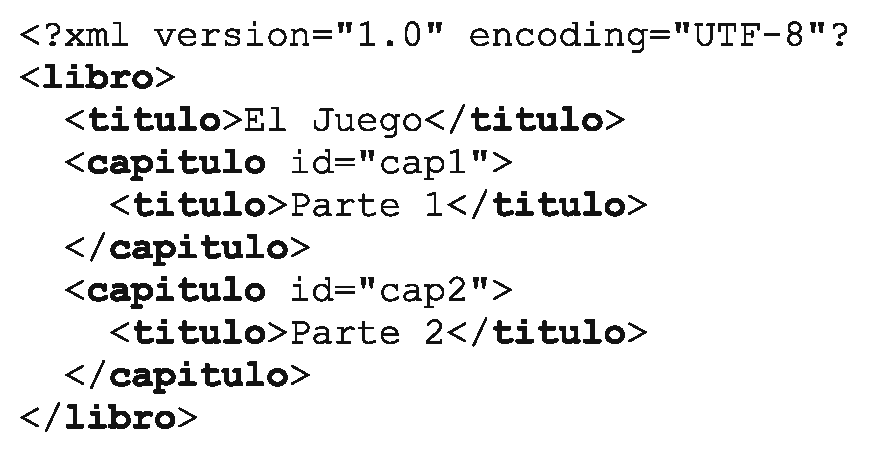
\includegraphics[scale=.5]{images/XML-document-example1}
%  \caption{\em Modelo de árbol para un documento XML.}
%  \label{fig:xml-tree-exa1}
%\end{figure}



